\documentclass{beamer}

\usepackage[T1]{fontenc}
\usepackage[utf8]{inputenc}
\usepackage{graphicx}
\usepackage{tikz}
\usepackage{epigraph}
\usepackage{txfonts}
\usepackage{hyperref}
\usepackage[outputdir=./out]{minted}

\usetikzlibrary{fadings}
\usetikzlibrary{shadows}
\usetheme[circularprogress=true]{BayooTec}
\usemintedstyle{one-dark}

% \definecolor{sourcebg}{HTML}{131a24}
\definecolor{sourcebg}{HTML}{232a34}

\newminted{ruby}{
  fontsize=\scriptsize,
  numbersep=8pt,
  gobble=4,
  bgcolor=sourcebg,
}

\title{Code is Music}
\subtitle{Eine Einführung ins Live-Coding}
\author{Martin Gondermann}
\date{01. Februar 2023}

\setlength{\epigraphwidth}{0.5\textwidth}

\newenvironment{colortheme}[1]{
  \input beamercolortheme#1.sty
}{}

\begin{document}

% Startseite
\begin{frame}[plain]
  \renewcommand{\epigraphflush}{center}
  \epigraph{
    \usebeamercolor{palette primary}
    \textbf{\textcolor{fg}{Live}} coding music, \\
    \textbf{\textcolor{fg}{Electronic}} notes dance and flow, \\
    \textbf{\textcolor{fg}{Algorithms}} sing.
  }{\usebeamercolor{palette secondary}\textcolor{fg}{\textit{Haiku by Chat GPT}}}
\end{frame}
\addtocounter{framenumber}{-1}

\begin{frame}[plain]
  \titlepage%
\end{frame}
\addtocounter{framenumber}{-1}

\begin{frame}
  \frametitle{Über mich}
  \begin{columns}
    \column{0.2\textwidth}
    \column{0.6\textwidth}
    \centering
    \begin{tikzpicture}
      \usebeamercolor{palette primary}\fill[fg, circular drop shadow={shadow scale=1.02,shadow xshift=0.6ex, shadow yshift=-0.6ex}] (0, 0) circle [radius=2cm];
      \clip (0, 0) circle (1.9cm);
      \node[anchor=center] at (0, 0) {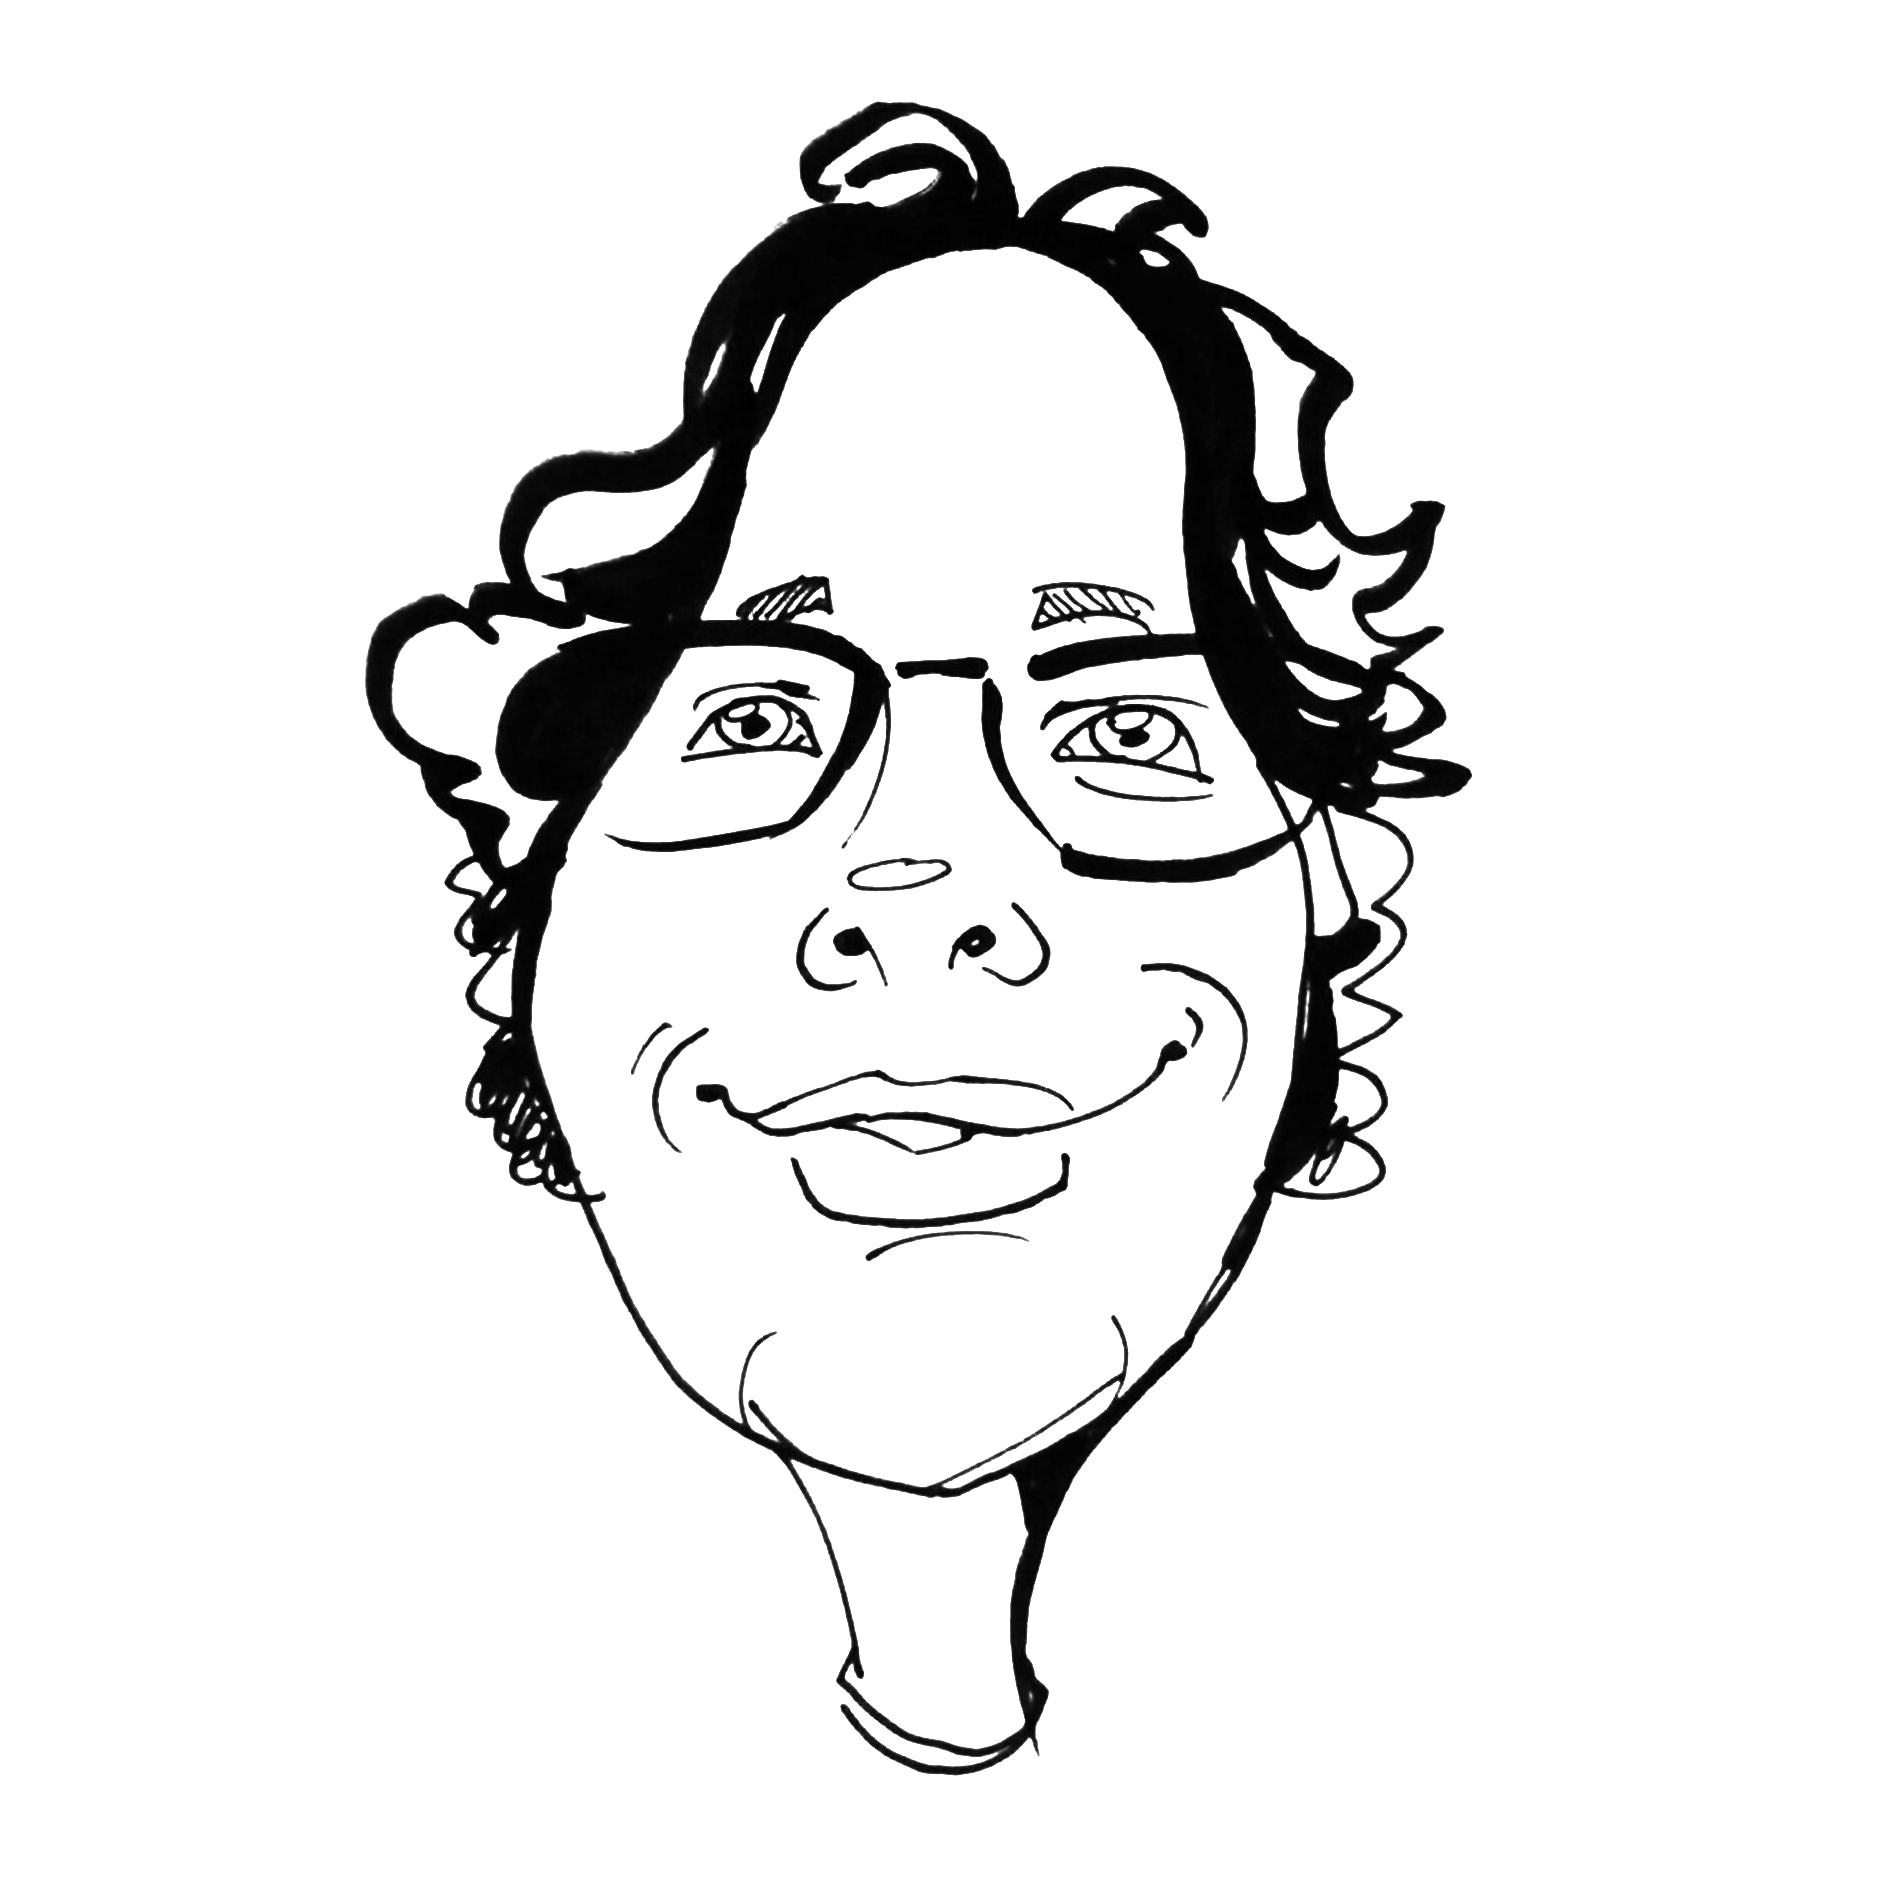
\includegraphics[width=3.9cm]{images/karikatur.png}};
    \end{tikzpicture}

    \vspace{0.5ex}
    \usebeamercolor[fg]{palette primary}\textbf{\textit{Martin Gondermann}}

    \usebeamercolor[fg]{palette secondary}\textit{Senior Software Engineer, Bayootec}
    \column{0.2\textwidth}
  \end{columns}
\end{frame}
\addtocounter{framenumber}{-1}

\begin{colortheme}{Lambdaphonic}
  \begin{frame}
    \frametitle{Über mich}
    \framesubtitle{The dark side}
    \usebeamercolor[fg]{palette primary}
    \begin{columns}
      \column{0.2\textwidth}

      \column{0.6\textwidth}
      \centering
      \begin{tikzpicture}
        \usebeamercolor{palette primary}\fill[fg, circular drop shadow={shadow scale=1.02,shadow xshift=0.6ex, shadow yshift=-0.6ex}] (0, 0) circle [radius=2cm];
        \clip (0, 0) circle (1.9cm);
        \usebeamercolor{background canvas}\fill[bg, circular drop shadow={shadow scale=1.02,shadow xshift=0.6ex, shadow yshift=-0.6ex}] (0, 0) circle [radius=1.9cm];
        \node[anchor=center] at (0, 0) {
\includegraphics[width=3cm]{images/lambdaphonic.png}};
      \end{tikzpicture}

      \vspace{0.5ex}
      \textit{$\lambda$phonic}

      \usebeamercolor[fg]{palette secondary}
      \textit{Live coder}

      \usebeamercolor[fg]{palette tertiary}
      \small\url{https://lambdaphonic.de}

      \column{0.2\textwidth}
    \end{columns}
  \end{frame}
\end{colortheme}

\section{Was ist Live Coding?}
\subsection{Definition}
\begin{frame}
  \frametitle{Was ist Live Coding?}
  \framesubtitle{Definition}
  The Live Coder creates and manipulates source code live in front of an audience.

  \vspace{1ex}
  He combines code, music and visuals into a synaestetic performance.
\end{frame}

\begin{frame}
  \frametitle{Was ist Live Coding?}
  \framesubtitle{TOPLAP}
  \small
  \begin{itemize}
    \item Give us access to the performer's mind, to the whole human instrument.
    \item Obscurantism is dangerous. Show us your screens.
    \item Programs are instruments that can change themselves
    \item The program is to be transcended --- Artificial language is the way.
    \item Code should be seen as well as heard, underlying algorithms viewed as well as their visual outcome.
    \item Live coding is not about tools. Algorithms are thoughts. Chainsaws are tools. That's why algorithms are sometimes harder to notice than chainsaws.
  \end{itemize}
\end{frame}

\section{Geschichte}
\begin{frame}
  \frametitle{Geschichte}
  \begin{itemize}
    \item 80er Jahre
      \begin{itemize}
        \item HMSL --- Forth basierte Sprache mit MIDI input/output
        \pause\item 1985: die erste dokumentierte Live Coding Performance: Ron Kuivila STEIM Amsterdam
      \end{itemize}
    \pause{}
    \item 2000+
      \begin{itemize}
        \item 2000: premiere von slub (Live Coding Band)
        \pause\item 2004: Gründung von TOPLAP \\ (\textbf{T}errestrial \textbf{O}rganisation for the \textbf{P}ragmatics of \textbf{L}ive \textbf{A}lgorithm \textbf{P}rogramming)
      \end{itemize}
  \end{itemize}
\end{frame}

\section{Live Coding Systeme}
\begin{frame}
  \frametitle{Live Coding Systeme}
  \framesubtitle{Eine Auswahl}
  \begin{columns}
    \column{0.5\textwidth}
    \begin{itemize}
      \item Supercollider
        \begin{itemize}
          \item Die ``Mutter'' der meisten Live Coding Systeme
        \end{itemize}
      \pause\item Gibber (Web / JavaScript)
      \pause\item Orca (Visual~``Programming'')
      \pause\item Tidal Cycles (Haskell~based)
      \pause\item Overtone (Clojure)
    \end{itemize}

    \column{0.5\textwidth}
    \begin{itemize}
      \pause\item GLICOL (Rust)
      \pause\item FoxDot (Python)
      \pause\item Extempore (Scheme~based)
      \pause\item \textbf{Sonic Pi (Ruby)}
    \end{itemize}
  \end{columns}
  \pause\centering
  \vspace{1em}
  \url{https://github.com/toplap/awesome-livecoding}
\end{frame}

\section{Sonic Pi}
\subsection{Basics}
\begin{frame}{Sonic Pi}{Basics}
  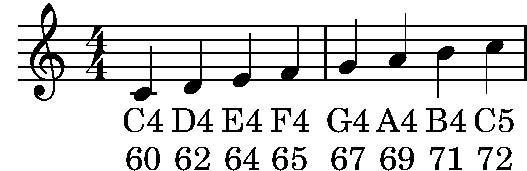
\includegraphics{images/scale.pdf}
\end{frame}

\defverbatim[colored]\playBasic{
  \begin{rubycode}
    # spielt die Note C4 mit dem aktuell ausgewählten Instrument
    play :C4
    play 60 # das Selbe, nur in MIDI notation
  \end{rubycode}
}

\defverbatim[colored]\playMulti{
  \begin{rubycode}
    # spielt mehrere Noten (Akkord) gleichzeitig
    play :C4
    play :E4
    play :G4
  \end{rubycode}
}

\defverbatim[colored]\playSleep{
  \begin{rubycode}
    # spielt die Noten nacheinander ab (1/4 Noten)
    play :C4
    sleep 0.25
    play :E4
    sleep 0.25
    play :G4
    sleep 0.25
  \end{rubycode}
}

\begin{frame}[fragile]{Sonic Pi}{Basics}
  \playBasic{}
  \pause\playMulti{}
  \pause\playSleep{}
\end{frame}

\defverbatim[colored]\envelopeReleaseExample{
  \begin{rubycode}
    play 60, release: 2
  \end{rubycode}
}

\defverbatim[colored]\envelopeAttackReleaseExample{
  \begin{rubycode}
    play 60, attack: 0.7, release: 2
  \end{rubycode}
}

\defverbatim[colored]\envelopeAttackSustainReleaseExample{
  \begin{rubycode}
    play 60, attack: 0.3, sustain: 1, release: 1
  \end{rubycode}
}

\defverbatim[colored]\envelopeAttackDecaySustainReleaseExample{
  \begin{rubycode}
    play 60,
      attack: 0.1, attack_level: 1,
      decay: 0.2,
      sustain: 1, sustain_level: 0.4,
      release: 0.5
  \end{rubycode}
}

\subsection{Hüllkurven}
\begin{frame}
  \frametitle{Sonic Pi}
  \framesubtitle{Hüllkurven}
  \centering
  \only<1>{
    \Large{Release}

    \vspace{2em}

    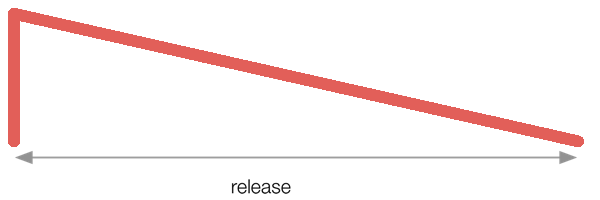
\includegraphics[width=0.5\textwidth]{images/env-release.png}

    \envelopeReleaseExample{}
  }
  \only<2>{
    \Large{Attack---Release}

    \vspace{2em}

    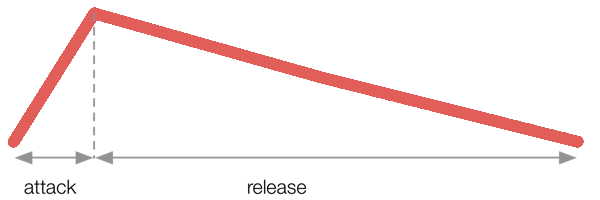
\includegraphics[width=0.5\textwidth]{images/env-attack-release.png}

    \envelopeAttackReleaseExample{}
  }
  \only<3>{
    \Large{Attack---Sustain---Release}

    \vspace{2em}

    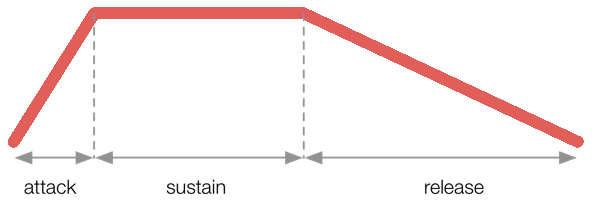
\includegraphics[width=0.5\textwidth]{images/env-attack-sustain-release.png}

    \envelopeAttackSustainReleaseExample{}
  }
  \only<4>{
    \Large{Attack---Decay---Sustain---Release}

    \vspace{2em}

    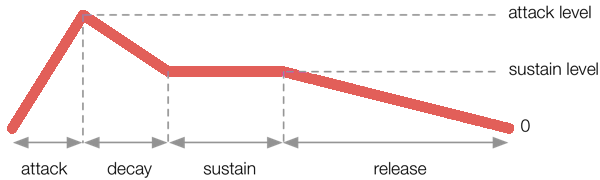
\includegraphics[width=0.5\textwidth]{images/env-attack-decay-sustain-release.png}

    \envelopeAttackDecaySustainReleaseExample{}
  }
\end{frame}

\subsection{Datenstrukturen}
\subsubsection{Listen}
\begin{frame}[fragile]
  \frametitle{Sonic Pi}
  \framesubtitle{Datenstrukturen --- Listen}

  \begin{rubycode}
    # Liste initialisieren
    notes = [:C4, :F4, :G4, :C3]
    notes = [60, 65, 67, 48]

    # Zugreifen
    puts notes[1] # gibt 65 zurück

    # Listen-Operatoren
    reversed = notes.reverse          # [48, 67, 65, 60]
    random_note = [60, 64, 67].choose # Zufälligen Eintrag auswählen
    two_notes = notes.pick(2)         # 2 zufällige Einträge
    shuffled = notes.shuffle          # Liste mischen (neue Liste)

  \end{rubycode}
\end{frame}

\subsubsection{Ringe}
\begin{frame}[fragile]
  \frametitle{Sonic Pi}
  \framesubtitle{Datenstrukturen --- Ringe}

  \begin{rubycode}
    values = ring(52, 55, 59)   # Ring erzeugen
    values = [52, 55, 59].ring  # Ring erzeugen aus Liste
    values[0]                   # erstes Element (52)
    values[2]                   # drittes Element (59)
    values[3]                   # Überlauf, wieder erstes Element (52)

    # Spezielle Ringe
    range(1, 5)              # ring(1, 2, 3, 4)
    range(1, 5, 0.5)         # ring(1, 1.5, 2, 2.5, 3, 3.5, 4, 4.5)
    bools(1, 0, true, false) # ring(true, false, true, false)
  \end{rubycode}
\end{frame}

\subsection{Zufall/Randomisierung}
\begin{frame}[fragile]{Sonic Pi}{Zufall/Randomisierung}
  \begin{rubycode}

    # Zufallswerte
    rand()          # Zufallszahl zwischen 0.0 und 1.0
    rand(0.5)       # Zufallszahl zwischen 0.0 und 0.5
    rand(0.1..0.8)  # Zufallszahl zwischen 0.1 and 0.8
    rand_i(5)       # Zufällige Ganzzahl (eine von 0, 1, 2, 3, 4)
    rdist(1, 0)     # Zufallszahl zwischen -1.0 und 1.0
    rrand(6, 10.5)  # Zufallszahl zwischen 6.0 und 10.5 inklusive
    rrand_i(6, 10)  # Zufällige Ganzzahl zwischen 6 and 10 inklusive
    dice            # würfelt (6-seitiger Würfel) (1-6 inklusive)
    dice(3)         # würfelt (3-seitiger Würfel)
    one_in(3)       # true mit Wahrscheinlichkeit von 1/3

  \end{rubycode}
\end{frame}

\subsubsection{Beispiele}
\begin{frame}[fragile]{Sonic Pi}{Zufall/Randomisierung --- Beispiele}
  \begin{rubycode}

    # zufällige Note des A-moll Akkords spielen
    play chord(:A4, :minor).choose

    # Sample mit einer Wahrscheinlichkeit von 50% (1/2) abspielen
    sample :drum_cymbal_pedal if one_in(2)

    # spielt das Sample mit einer zufälligen Lautstärke
    sample :drum_cymbal_pedal, amp: rand(0.4..0.8)

  \end{rubycode}
\end{frame}

\subsection{Samples}
\begin{frame}[fragile]{Sonic Pi}{Samples}
  \begin{rubycode}
    # sample abspielen
    sample :loop_amen
    sample :loop_amen, rate: 0.5 # halbe Geschwindigkeit
    sample :loop_amen, rate: -1  # rückwärts

    # Anpassung der Sample-Länge
    sample :loop_amen, beat_stretch: 2

    # Pitch-Anpassung
    sample :bass_trance_c, rpitch: 2

    # mit Hüllkurve
    sample :loop_amen, attack: 0.25, release: 0.25

    # partielle Samples
    sample :loop_amen, start: 0.4, finish: 0.6
    sample :loop_amen, start: 0.6, finish: 0.4

  \end{rubycode}
\end{frame}

\begin{frame}
  \usebeamercolor{palette primary}
  \centering
  \textbf{\textcolor{fg}{\Huge{Demo}}}
\end{frame}

\begin{frame}
  \usebeamercolor{palette primary}
  \centering
  \textbf{\textcolor{fg}{\Huge{Vielen Dank!}}}
\end{frame}

\end{document}
